% Copyright (c) 2010 Jérémie DECOCK (http://www.jdhp.org)

\documentclass[pdftex,a4paper,11pt]{article} 
\usepackage[utf8]{inputenc}
\usepackage[frenchb]{babel}
\usepackage[pdftex]{graphicx}
\usepackage{hyperref}

\hypersetup{
    pdftoolbar=true,                                          % show Acrobat’s toolbar ?
    pdfmenubar=true,                                          % show Acrobat’s menu ?
    pdffitwindow=true,                                        % page fit to window when opened
    pdftitle={Maquettes},                                     % title
    pdfauthor={Jérémie DECOCK},                               % author
    pdfsubject={Maquettes},                                   % subject of the document
    pdfnewwindow=true,                                        % links in new window
    pdfkeywords={},                                           % list of keywords
    colorlinks=true,                                          % false: boxed links; true: colored links
    linkcolor=black,                                          % color of internal links
    citecolor=black,                                          % color of links to bibliography
    filecolor=black,                                          % color of file links
    urlcolor=black                                            % color of external links
}

\begin{document}

\title{OpenCAL - Java\\\medskip
       Maquettes}
\author{Jérémie \bsc{Decock}}
\date{\today}

\maketitle

%%%%%%%%%%%%%%%%%%%%%%%%%%%%%%%%%%%%%%%%%%%%%%%%%%

\section{Introduction}

L'interface est découpé en 5 panneaux, répondant chacun à un cas d'utilisation :
\begin{itemize}
    \item créer de nouvelles cartes;
    \item tester régulièrement ses connaissances sur un ensemble de cartes;
    \item réviser un ensemble de cartes choisi;
    \item modifier les cartes de sa base personnelle;
    \item contrôler sa progression et son assiduité sur les cartes testées;
\end{itemize}

\section{Maquettes}

TODO : mettre ici les captures des maquettes faites sur papier puis scannés (ne pas utiliser Glade ou équivalant, c'est trop lent et inefficace : peu de widgets, on peut pas personnaliser les widgets, etc.).

%\begin{figure}[htbp]
%    \centering
%    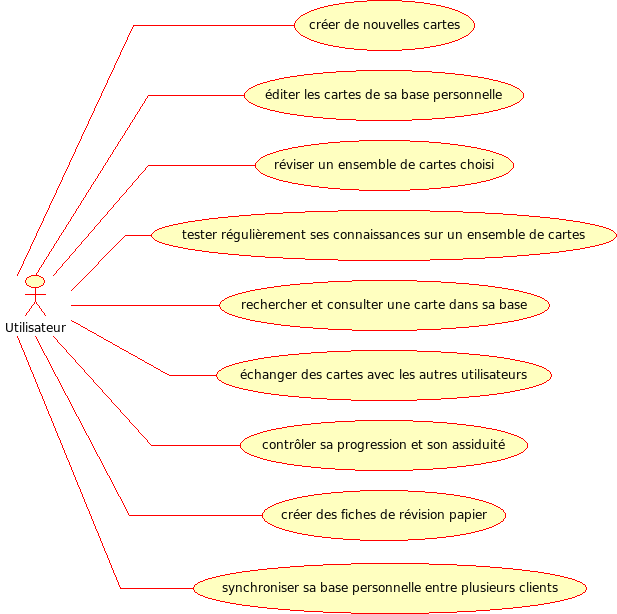
\includegraphics[width=10cm]{fig/use_case_diagram}
%    \caption{Cas d'utilisation de l'application}
%    \label{use_case}
%\end{figure}

\section{Principaux menus de l'application}

\begin{small}
\begin{tabular}{|p{0.2\textwidth}|p{0.4\textwidth}|p{0.4\textwidth}|}
    \hline
    Menu & Élément & Description\\
    \hline
    \hline
    File / Fichier & New... / Nouveau... & Créer une nouvelle base personnelle \\
    \cline{2-3}
                   & Open... / Ouvrir... & Ouvrir une base personnelle existante\\
    \cline{2-3}
                   & Close / Fermer      & Fermer la base personnelle courante\\
    \cline{2-3}
                   & Inport Card Set... / Importer un ensemble de cartes...   & Importer un ensemble de cartes \\
    \cline{2-3}                                                                                             
                   & Export Card Set... / Exporter un ensemble de cartes...   & Exporter un ensemble de cartes \\
    \cline{2-3}
                   & Export Review File... / Créer une fiche de révision...   & Créer une fiche de révision \\
    \cline{2-3}                                                                                                
                   & Print Review File... / Imprimer une fiche de révision... & Imprimer une fiche de révision \\
    \cline{2-3}
                   & Exit / Quitter & Quitter l'application \\
    \hline
    Edit / Édition & Undo / Annuler & Annuler la dernière opération \\
    \cline{2-3}
                   & Redo / Refaire & Refaire la dernière opération \\
    \cline{2-3}
                   & Cut / Couper   & Couper la sélection courante \\
    \cline{2-3}
                   & Copy / Copier  & Copier la sélection courante \\
    \cline{2-3}
                   & Paste / Coller & Coller la sélection courante \\
    \cline{2-3}
                   & Delete / Supprimer & Supprimer la sélection courante \\
    \cline{2-3}
                   & Preferences... /Préférences...    & Modifier les préférences \\
    \hline
    Help / Aide    & OpenCAL Help... / Aide OpenCAL... & Afficher la page d'aide \\
    \cline{2-3}
                   & About... / À propos de... & Afficher les copyrights \\
    \hline
\end{tabular}
\end{small}

%%%%%%%%%%%%%%%%%%%%%%%%%%%%%%%%%%%%%%%%%%%%%%%%%%

\clearpage

\begin{center}
    Copyright \textcopyright{} 2010 Jérémie \bsc{Decock}.\\
    All right reserved.
\end{center}

\end{document}

